\chapter{Experiments: Optomechanics}
% References are needed for historical context, technical claims, and specific data.
% Suggested [?] placements below:

This chapter will cover the experimental methods used in the development of optomechanical three-mirror cavity systems, focusing on the design, fabrication, and characterization of mechanical resonators within optical cavities. The methods are designed to enhance the sensitivity of measurements in quantum optics and optomechanics.
\minitoc
\newpage 

Over the past two decades, optomechanical systems have greatly benefited from advancements in optical coating technologies, enabling the realization of high-finesse cavities ($\mathcal{F}>10^5$)\cite{coating_review}. Simultaneously, progresses in micro/nanofabrication allowed the making of mechanical structures with high $Q$ factors ($>10^6$)\cite{nanofab_review}. Despite these achievements, a significant challenge remained: fabricating mechanical elements that possess both high $Q$ and high reflectivity, as optical, mechanical and thermal effects often degrade system performance and hinder ultra-sensitive measurements\cite{optomech_challenges}.
\section{System Description and Setup}

\subsection{Previous LKB work and Motivation}

Previous optomechanics experiments at LKB have primarily utilized Fabry--Pérot cavities with two mirrors, where the end mirror of the cavity was typically a HR mirror deposited on top of a mechanical structure featuring a mechanical mode of interest~\cite{}. \\

Over Aurélien's and Leonard's PhD works, the group in collaboration with ONERA developed a platform based on a $1$-mm-thick quartz micropillar with an effective mass of $33~\mu$g. The structure supports a fundamental compression mode oscillating at $3.6$~MHz, with a mode shape as shown in Fig.~\ref{fig:micropillar_mode}. Using a dry-film photoresist technique, a $100~\mu$m diameter high-reflectivity mirror was deposited on one end of the pillar. Careful design of the suspension has yielded mechanical quality factors up to $3\times 10^{6}$ at room temperature and up to $7\times 10^{7}$ below 1~K. When integrated into a $50~\mu$m-long Fabry--Pérot cavity with a custom-fabricated coupling mirror, finesses exceeding $10^{5}$ were achieved. Importantly, this compact cavity remains robust against vibrations of the dilution refrigerator and maintains alignment during cooldown, thereby providing a stable platform to study optomechanical effects in the intermediate mass regime. \color{red} limitations and why it didnt work \color{black} \\

Then over Rémi's and Michael's PhD, another resonator was developed in collaboration with Francesco Marin’s team, based on a suspended silicon disk. The device operates in a balanced mode, where the central disk vibrates in opposition to four surrounding counterweights. By adjusting the geometry, the resonance frequency was increased to $280$~kHz, corresponding to an effective mass of about $110~\mu$g, bringing the system closer to the micropillar parameters. A HR mirror was then deposited on top using the same technique as the micropillar. Finesse of about $\sim 50 000$ were then reached. At cryogenic temperature, optimized designs reached mechanical quality factors on the order of $1.2 \times 10^{6}$.\color{red} limitations and why it didnt work \color{black} \\

Although the systems ended up being limited by various factors mentioned above (optical, mechanical and thermal effects)~\cite{}, the parts designed over the years did feature a high level of passive stability as well as good thermalization properties.  A pivotal solution, introduced by Regal, Kimble, Harris, and collaborators\cite{Regal2008,Harris2008}, was to decouple these requirements by embedding a high-$Q$ mechanical resonator within a high-finesse optical cavity, using the optical field to probe and control the resonator’s dynamics.

\subsection{Specifications and Design}
It was then decided to build on this design and extend it to a three-mirror cavity in a MATE configuration to benefit from this large linear and tunable coupling range as detailed in the previous chapter. That is the work Michael and myself undertook during my M2 internship and the following years of my PhD.
This new three mirror cavity then needed to fulfill various requirements detailed in what follows. 

\subsubsection{High Finesse} 

Low loss mirrors were produced by \textbf{Jérôme~DEGALLAIX} and \textbf{David~HOFMAN} at the
\textit{Laboratoire des Matériaux Avancés} (LMA, Lyon) using
ion-beam-sputtered (IBS) Bragg stacks made of $\mathrm{Ta_2O_5}$ (high index,
$n\!\approx\!2.09$) and $\mathrm{SiO_2}$ (low index, $n\!\approx\!1.46$)\cite{AmatoPhD,LMA_IBS}. The coatings were deposited in the LMA's \textit{Veeco SPECTOR} chambers and subsequently annealed at 500°C for 10 hours to minimise both optical (absorption) and mechanical losses, following the recipe of Amato \textit{et~al.}\,\cite{AmatoPhD}.
\footnote{Identical optics are used for the Advanced LIGO, Advanced Virgo
and KAGRA interferometers\cite{LIGO_optics}.}.\\

We supplied the LMA with a batch of substrates with various radii of curvature to explore different cavity geometries. The requested specifications are summarized in the table below. The total round‐trip scatter and absorption losses are usually below $ 20\,$ppm, in agreement with the measurements reported (absoption $\sim$0.7ppm, scattering $\sim$10ppm)in Ref.\,\cite{AmatoPhD}.


\begin{table}[h!]
\centering
\begin{tabular}{lcccc}
\textbf{Substrate type} & \textbf{Laseroptik ID} & \textbf{$R$} &
\textbf{Front-side HR $T$} & \textbf{Back-side AR} \\
\hline
Plane         & S--00798 & $\infty$ (plane) & $20 \pm 45$ ppm        & $R \lesssim 100$ ppm \\
Plano-concave & S--00128 & -25 mm           & $100,\,50 \pm 10$ ppm  & $R \lesssim 100$ ppm \\
Plano-concave & S--00127 & -15 mm           & $100,\,50 \pm 10$ ppm  & $R \lesssim 100$ ppm \\
Plano-concave & S--00126 & -10 mm           & $100,\,50 \pm 10$ ppm  & $R \lesssim 100$ ppm \\
\end{tabular}
\caption{Specifications of supplied Laseroptik substrates for different cavity geometries.}
\end{table}

The quarter‐wave design is centred at $\lambda = 1064$ nm for normal incidence.  After annealing, the measured mechanical loss angle of the $\mathrm{TiO_2\!:\!Ta_2O_5}/\mathrm{SiO_2}$ stack is $\phi < 4\times10^{-4}$ at 1 kHz  \color{red} link to mechanical damping needed \color{black}, supporting cavity finesses in the range $200\,000-500\,000$ before excess scatter or absorption dominates\cite{AmatoPhD}. 

\subsubsection{High $Q$ factor} 

Two different square membranes were used in the MATE cavities, both made of high-stress silicon nitride (Si$_3$N$_4$), a material known for its excellent mechanical properties, including high tensile stress and low intrinsic mechanical loss, making it ideal for optomechanical applications\cite{SiN_review}, and of nominal side lengths $l_n \times l_m = 500\,\mu m\times500\,\mu m $. \\ 

The first membrane was made in-house at LKB by \textbf{Thibaut Jacqmin} and \textbf{Himanshu Patange} during Himanshu's PhD work. The silicon wafer was 350 $\mu$m thick, and the SiN layers thicknesses was nominally 100 nm. Starting with the silicon wafer/chip coated with SiN on both sides, a photoresist is patterned by lithography to define a square window. Reactive-ion etching (RIE) then opens a square window through the top SiN layer. The exposed silicon is then wet-etched in KOH from the opened side until the cavity breaks through, leaving a released, free-standing SiN membrane spanning the opening. The membrane is then cleaned using HF to remove any residuals from the fabrication process. This very process etches the SiN layer as well, resulting in a final membrane thickness of less than 100nm. For detailed fabrication steps, refer to Himanshu's PhD thesis\cite{PatangePhD}. We nonetheless succintly display the fabrication steps in Fig \ref{fig:plain_sin_fab}. \\ 


\begin{figure}
    \centering  
    \includegraphics[width=\textwidth]{./chap5/fig/plain_sin_fab.pdf}
    \caption{Fabrication steps of the SiN membrane resonator used in the MATE cavity. (a) starting from a silicon wafer coated with SiN on both sides. (b) lithography and RIE to open a square window in the top SiN layer. (c) KOH wet etching from the opened side until the cavity breaks through, leaving a free-standing SiN membrane. The membrane is then cleaned using HF to remove any residuals from the fabrication process.}
    \label{fig:plain_sin_fab}    
\end{figure}


The second membrane is a commercially Norcada\textsuperscript{\textregistered} (NX10050AS)\cite{SiN_review,Norcada_datasheet} SiN square membrane, specifically marketed as a \textit{high Q} standard membrane for optomechanics applications. It features a Silicon frame of 200 $\mu$m thickness, and a SiN layer of nominal thickness 50 nm. Regarding the quality factor, literature reports:
\begin{itemize}
  \item \textbf{Room temperature.}  Measurements on nominally identical
        Norcada membranes report quality factors
        $Q \sim 5\times10^{6}$ at $\approx1\,\mathrm{MHz}$ in
        $<10^{-6}$ mbar vacuum \cite{SiN_review,Norcada_datasheet}.
  \item \textbf{Cryogenic operation.}  Cooling to $T \lesssim 300\,\mathrm{mK}$
        reduces internal friction by an order of magnitude, with
        $Q>10^{7}$ routinely observed \cite{SiN_cryogenic}.
\end{itemize}

The membrane’s high stress, thin-film nature and dielectric composition make
it fully compatible with ultra-high-vacuum environments and repeated
cryogenic cycling, while introducing (a priori) negligible optical loss in the cavity.
The expected mechanical mode structure can be derived from 
\begin{equation}
f_{n,m}= \sqrt{\dfrac{\sigma}{4\rho}\left(\left(\dfrac{n}{l_n}\right)^2+\left(\dfrac{m}{l_m}\right)^2\right)}
\end{equation}
with $\rho \sim 3 \,\mathrm{g/cm^3}$ the film mass density, $\sigma \sim 1 \text{GPa}$, ($n,m$) the mode indices, and ($l_n,l_m$) the membrane side lengths. Considering a square membrane of identical side lengths of $500\mu m$ yields a fundamental mode frequency at $f_{1,1} \sim 816\,\mathrm{kHz}$, with the two higher order modes $(1,2)$ and $(2,1)$ degenerate at $f_{1,2}\sim f_{2,1} \sim 1.29\,\mathrm{MHz}$ etc.. We display the first few mode shapes and expected frequencies in Fig.~\ref{fig:simumode}. 
 \begin{figure}
    \centering  
    \includegraphics[width=\textwidth]{./chap5/fig/simumode.pdf}
    \caption{Simulated mode shapes and frequencies of a square SiN membrane of side length $500\mu m$ under high tensile stress ($\sigma \sim 1 \text{GPa}$).}
    \label{fig:simumode}
\end{figure}

\subsubsection{Optical alignement}
 The cavity is designed to be compatible with the Thorlabs\textsuperscript{\textregistered} cage system. The input mirror is mounted on a 3 axis cage mount, allowing for easy alignment of the input mirror with respect to the cavity optical axis. Both the resonator and the back mirror are embedded within a custom-made holder, which is itself integrated into the cage system. The relative tilt between the resonator and the back mirror is adjusted using a set of 3 screws with a very fine thread, allowing for a fine alignment of the parallelism of the back cavity. The alignment procedure is detailed in section~\ref{sec:alignment_procedure}.





\subsubsection{Dynamical range}

The input mirror is glued to a PI Ceramic\textsuperscript{\textregistered} \texttt{P-016.00H} ring-stack piezoelectric actuator using vacuum epoxy (Torr Seal\textsuperscript{\textregistered}). Driven from 0 to $+1000\,\mathrm{V}$ it provides a longitudinal stroke of $5\,\mu\text{m}$, a blocking force of $2.9\,\mathrm{kN}$, as well as an unloaded resonance of 144 kHz, making it suitable for fast, low-noise cavity-length control. \\

The end-mirror–membrane assembly is mounted on a custom holder actuated by three \texttt{PD080.31} piezo chips arranged mechanically in series. Each chip yields $2\,\mu\text{m}$ of travel over a drive range of $-20$ to $+100\,\mathrm{V}$; the triple stack therefore supplies roughly $6\,\mu\text{m}$ of coarse tuning while preserving high stiffness and sub-microsecond response. The effective range is lower than this owing to the fact the piezo is constrained within the holder. Furthermore, one should not constrain the piezo to much to avoid damaging it: it happened that the assembly was too tightly screwed in such that it ended up fracturing the piezo pushing against the back mirror holder. An easy workaround would be to add some elastic spacer between the piezo and the copper piece (like kapton tape for example). \\ 

Combining the $5\,\mu\text{m}$ stroke of the front \texttt{P-016.00H} with the $6\,\mu\text{m}$ range of the rear triple stack provides an overall cavity-length adjustment sufficient to scan few FSRs, as well as to tune the membrane position over a full wavelength, thus accessing allowing exploration of the three mirror cavity physics.


\subsubsection{Compactness \& Stability}
The entire assembly is built as a cage system using standard Thorlabs\textsuperscript{\textregistered} cage parts, allowing for a compact and stable assembly. The cage system also allows for (relatively) easy alignment of the mirrors, as well as easy access to the piezo actuators.

\subsubsection{Vacuum and Cryogenic compatibility}
The back cavity composed of the back mirror and the middle mirror is embedded inside an Oxygen Free Copper (OFHC) assembly with a circular geometry, eventually mitigating for transverse misalignment issues when going to cryogenic temperatures, the constraints compensating themselves radially with respect to the symmetry axis of the cavity assembly\cite{OFHC_review}. Furthermore, the screws used to hold the assembly together are made of brass with a thermal expansion coefficient lower than that of the OFC, tightening up the cavity when reaching cryogenic temperatures.
Thorlabs cage parts are compatible with moderate vacuum operation down to $\sim 10^{-7} \text{mbar}$ if properly degreased and ultrasound cleant, but a custom cryocompatible system to hold the input mirror would be needed for operation at cryogenic temperatures. \\


\begin{figure}
    \centering  
    \includegraphics[width=\textwidth]{./chap5/fig/schéma_cavity.pdf}
    \caption{Cavity design and assembly. (a) The figure shows the overall assembly of the MATE system from various views, highlighting the integration of the high-finesse mirrors, the membrane resonator embedded inside the back cavity copper assembly held to the input mirror Thorlabs holder through a cage system.(b) The exploded view details the arrangement of the mechanical and optical components, illustrating the modular design that facilitates alignment, stability, and compatibility with vacuum environments.}
    \label{fig:cad_cavity}
\end{figure}


The initial design of the cavity was made using Autodesk Fusion 360, allowing for a detailed 3D model of the entire assembly, including the piezo actuators, the mirrors and the cage system. The design was then exported to a STEP file format, which was used to manufacture the parts using a 3 axis CNC milling machine and a digital lathe. The pieces were machined by \textbf{Carounagarane~DORE} and \textbf{Gael~COUPIN} at the LKB mechanical workshop with 100$\mu$m tolerance. A detailed view of the cavity design and assembly is shown in Fig.~\ref{fig:cad_cavity}.

\subsection{Flexure Actuation}

One specificity of the MATE system is that the back cavity is significantly shorter than the front cavity, which would require high precision in both the machining of the copper pieces and the positioning of the resonator. In our case, we aim at a centimetric cavity which would require to position the membrane at roughly hundreds of microns from the back mirror, and parallel to the back mirror. Moving the membrane independently from the back mirror while maintaining a controllable tilt between both planes is therefore challenging. \\


A smart workaround was introduced by Jack Sankey and its group \cite{Sankey2010}, where the authors introduced a flexure-tuned MATE system. The key innovation lies in actuating the membrane position by flexing its supporting silicon frame rather than translating the entire mount. This is done by mounting the back cavity in a semi-monolitic fashion, and 'locking' the silicon frame of the membrane using three screws with a fine thread, allowing for a fine adjustment of the angle of the membrane plane with respect to the back mirror plane. The piezos pushing on the back of the assembly then force the silicon frame constrained by the screws to bend, thus displacing the membrane with respect to the back mirror, as shown in Fig.~\ref{fig:flexure tune}. 
This approach preserves the cavity alignment for gentle flexures, while enabling continuous and wide-range tuning of both the membrane displacement and tilt. 


\begin{figure}[H]
    \centering  
    \includegraphics[width=\textwidth]{./chap5/fig/flexure tune.pdf}
    \caption{Cavity design and assembly. (a) In this configuration (no voltage applied to the piezos), the screws are used to align the membrane plane with respect to the back mirror plane, ensuring a good parallelism between both planes. (b) Flexure tuning of the membrane position. When a voltage is aplied to the piezos, they push on the back of the assembly, forcing the silicon frame to bend, thus displacing the membrane with respect to the back mirror. The two dashed lines show the initial positions of the back mirror and the membrane. This push shortens the overall cavity length (i.e. increasing the overall system's frequency), as well as the relative distance between the mirror and the membrane (i.e. changing the optomechanical coupling). }
    \label{fig:flexure tune}
\end{figure}


\color{black}

\subsection{Experimental Setup}
The assembly is now to be integrated into the optical setup shown in Fig.~\ref{fig:optical layout}. The source laser is a 1064nm Nd:YAG laser (Coherent Mephisto). We did not require the full optical power delivered by the laser, so a short optical path not detailed here splits the laser in 3 arms to eventually fiber couple some laser power and bring it to other experiments that would need 1064nm laser light. \newline

\begin{figure}[h!]
    \centering  
    \includegraphics[width=\textwidth]{./chap5/fig/fig_lock_MATE.pdf}
    \caption{}
    \label{fig:optical layout}
\end{figure}
The optical path then consists of : 
\begin{itemize}
  \item a first half waveplate and a beam splitter to adjust the total power injected into the experimental setup,
  \item a fibered electro-optics phase modulator (EOM Photline NIR-MPX-LN-10) to generate sidebands for the PDH locking of the cavity. It is polarization matched by using a fibered polarization controller to avoid Residual Amplitude Modulation noise (RAM) at the output (three blue circles on the optical layout). 
  \item a fiber coupler to go from a guided optical mode to a free space optical mode, with a the coupler adjusted such that the outputted beam is collimated and has a waist of about 1mm,
  \item a quarter waveplate to compensate for ellipticity of the output beam polarization, then a half waveplate and a beam splitter to adjust the powers injected into the cavity path and the prospective LO path, respectively,
  \item on the cavity path, a faraday rotator to ensure the cavity reflected beam to be deflected to an output port and not back into the fiber 
  \item a lens to mode match the laser input mode to the cavity mode, with a focal length of 40 to 60mm depending on the input mirror radii of curvature. This lens is mounted on a x-y cage system translation mount, and is mounted inside the vacuum chamber that features AR coated windows to allow for optical access yet minimal parasite reflections.
  \item the cavity itself. 
  \item two photodiodes (Thorlabs ???) to detect the reflected beam and the transmitted beam, respectively, with 40mm focal length lenses to focus the beam onto the photodiodes. 
\end{itemize}

The optical path was designed to be as modular as possible, allowing for easy replacement of the components if needed, as well as additions of optical elements. For this reason, it features two fainted additional optical paths as seen on Fig.~\ref{fig:optical layout}, one for a prospective LO, and another to deflect the reflected beam to a Homodyne Detection setup using a flip mirror. Polarization optics would aslo need to be added on the Homodyne Detection path to mix the LO and the reflected beam, but this was not done during this thesis.

\subsection{Alignment Procedures}
The optical setup is now to be aligned as to ensure a good mode matching between the laser input mode and the cavity mode. The steps are as follows, and the associated diagrams are shown in Fig.~\ref{fig:tilt}:
\begin{itemize}
  \item \textbf{Step 1} (Fig.~\ref{fig:tilt}(a))\textbf{:} we position an iris diaphragm before our two injection mirrors mounted on ($\theta_x$,$\theta_y$) kinematic mounts. We then adjust the tilt of both mirrors i.e. \textit{beam-walking}, such that the reflected beam is centered on the iris diaphragm: this is done by maximising the reflected signal on the reflection photodiode. This ensure the beam reflected by the output mirror (HR mirror) is at normal incidence. In a second time we tune the plane of the resonator using the three screws of the assembly. We monitor the Fizeau fringes in transmission with a camera (Allied Vision Alvium), and adjust the tilt such that no fringes are to be seen. 
  \item \textbf{Step 2} (Fig.~\ref{fig:tilt}(b))\textbf{:} we then place the focusing lens in the optical path, and adjust its position such that we recover maximal power on the reflection photodiode. This lens is mounted on the (x-y) cage system translation mount, and positioned at a distance from the back mirror fixed by the cavity mode matching requirements (ref chap theory). The lens is then fixed in place using the cage system screws.
  \item \textbf{Step 3} (Fig.~\ref{fig:tilt}(c))\textbf{:} we add the input mirror on a ($\theta_x$,$\theta_y$) cage system mount, and adjust its position to get an input beam normal to the tangent of the concave mirror curvature. This is also done maximising the reflected power on the reflection photodiode. The mount (and thus the mirror) was also positioned at the appropriate distance from the back mirror to ensure optimal mode matching. 
  \item \textbf{Step 4} (Fig.~\ref{fig:tilt}(d))\textbf{:} We scan the cavity length using the piezo actuator mounted on the input mirror, and monitor the cavity resonances using both the reflected and transmitted photodiodes. We finally fine tune the mode match by \textit{beam-walking} the two injection mirrors. We can also play with the collimating lens at the fiber coupler (not shown on the diagram) as to fine tune for longitudinal mode matching. The cavity is now aligned and ready for operation.
  \end{itemize}

\begin{figure}[h!]
    \centering  
    \includegraphics[width=\textwidth]{./chap5/fig/tilt_alignementB.pdf}
    \caption{Set up alignment procedure. (a) to (d) show the steps to align the cavity with respect to the optical path (detailed in the main text). The (a.i) to (a.iv) show what is seen on the camera for four different tilt positions where (a.iv) displays a 'good' tilt alignement: no visible fringes except for the dim fringes of the camera setup. These dim fringes are present when the beam is a normal incidence with the back mirror (use of the iris) and are believed to be intereferences arising from reflections inside the camera objective as they are seen whatever the plane of focus is. }
    \label{fig:tilt}
\end{figure}
\section{Experimental Characterization}
\subsection{Cavity Scans}

\begin{table}[h!]
    \centering
    \begin{tabular}{lcc}
         & Cavity I & Cavity II \\
        \hline
        Input mirror RoC (mm)        & \multicolumn{2}{c}{-25} \\
        Back mirror RoC (mm)         & \multicolumn{2}{c}{$\infty$} \\
        Nominal input mirror $T_1$ (ppm) & \multicolumn{2}{c}{100} \\
        Nominal back mirror $T_2$ (ppm)  & \multicolumn{2}{c}{20} \\
        Length $L$ (mm)               & 17 & 24 \\ 
        FSR (GHz)                  & 8.817 & 6.246  \\[0.6em]
        
    \end{tabular}
    \caption{Summary of relevant parameters for the two cavities used in this work.}
    \label{tab:mate_parameters}
\end{table}
 
Once the cavity is aligned, we can scan the cavity length by driving the front mirror piezo with a triangular or a sine wave voltage. This signal is first amplified using a high voltage amplifier made by the LKB electronic workshop, which can deliver up to 1000V. The output impedance of the amplifier is a standard 50 Ohms, but the piezo in parallel at the end of the line with capacitance of about 15 nF low pass filters the signal at  $\sim$ 200 Hz. We can also modulated the back piezo actuators, in DC or AC, and a similar lowpass filtering occurs with a lower cutoff frequency $\sim$ 50Hz (3 piezo actuators in parallel with a capacitance of around 100 nF each). \\ 

We then monitor the cavity resonances using both the reflected and transmitted photodiodes and scanning the cavity over a large range, as to mode match the cavity to the TEM$_{00}$ mode. By beam walking, we optimally mode match the cavity such that higher order modes vanish in the photodiode noise floor and the reflected and transmitted signals are maximised, we can then perform finer scans to characterize the cavity parameters. We observed that putting the cavity under vacuum did sometimes misalign the cavity, such that even mode matching to our best ability using two mirrors outside the vacuum tank did not yield a perfect $\text{TEM}_{00}$ match. We also saw some membranes/phononic crystals break throughout the pumping process, most likely due to dust or degazing of the setup. \\

Once aligned and mode matched, we can proceed to the cavity characterization. Over the course of my PhD, few \textit{functional} cavities were mounted inside the vacuum tank. We chose to only present the results for two of these, as to display various physical effects observed. The key parameters of these two cavities are summarized in Table~\ref{tab:mate_parameters}. Both were mounted using 100ppm input mirrors, with a concave radius of curvature of -25mm, and a plane back mirror with a nominal transmission of 20ppm. Cavity I used the in-house fabricated membrane of nominal thickness 100nm, while cavity II used the commercial Norcada membrane of nominal thickness 50nm. The reason why we used the 100ppm input mirror rather than the 50ppm one was to ensure that the cavity linewidth would be larger than the mechanical resonance frequency of the membrane, such that we would be in the genuine unresolved sideband regime. Had we chosen the 50ppm mirror, the cavity linewidth would have been around 85kHz, an order of magnitude below the expected fundamental mechanical resonance frequency of the membrane at 861kHz (see above). A tradeoff is to be made here, as using a higher transmission input mirror reduces the intracavity power for a given input power, thus reducing radiation pressure effects. 

\subsubsection{Cavity resonances versus membrane position } 
We first scan the input mirror piezo with a linear ramp $V_{\rm SW}$ ranging from 0 to 500V at 10-50Hz, corresponding to a displacements of around 2$\mu m$ ($\sim$ 4 FSRs). The back piezo actuating the membrane position was driven by a DC voltage $V_{\rm DC}$ ranging from 0 to 70V, with an associated stroke of 4$\mu m$ (3 piezos). Knowing the FSR of the cavity, we calibrate the piezo displacement as a function of the applied voltage, and fit the resonances positions using the theoretical model detailed in chapter 3. We modelled the front cavity length $L_1$ as well as the back cavity length $L_2$ as third order polynomials of the applied voltages $V_{\rm SW}$ and $V_{\rm DC}$  such that
\begin{equation}
  \begin{split}
    L_1 &= a_0 + a_1 V_{\mathrm{SW}} + a_2 V_{\mathrm{SW}}^2 + a_3 V_{\mathrm{SW}}^3 - \alpha V_{\mathrm{DC}}\\
    L_2 &= b_0 + b_1 V_{\mathrm{DC}} + b_2 V_{\mathrm{DC}}^2 + b_3 V_{\mathrm{DC}}^3
  \end{split}
\end{equation} 
where we introduced the coefficients $a_i$ and $b_i$ to be fitted, as well as a cross-coupling term $\alpha V_{DC}$ to take into account the fact that the back piezo actuators does change the front cavity length since the piezo pushing the back cavity assembly bends the silicon frame. \\

\begin{figure}[h!]
    \centering  
    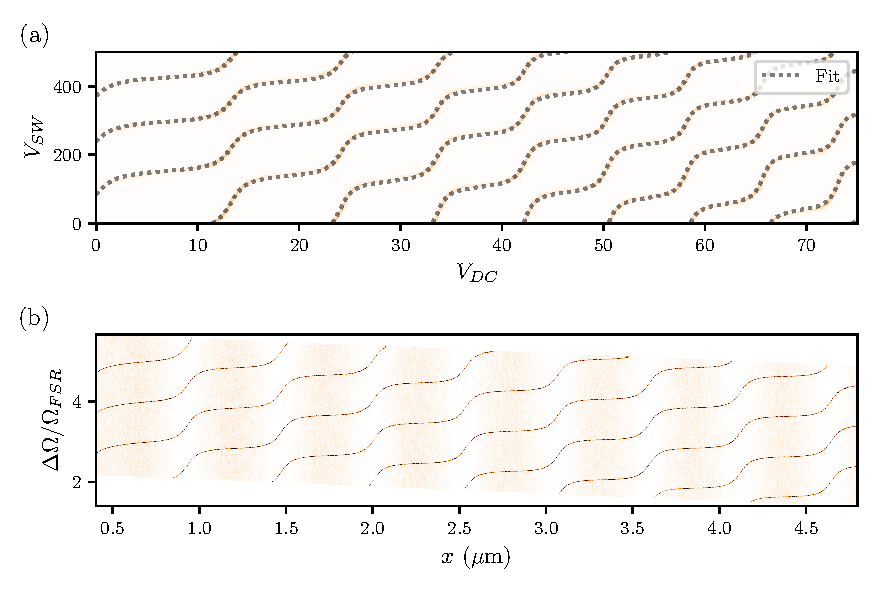
\includegraphics[width=\textwidth]{./chap5/fig/scansTot.pdf}
    \caption{Scans of cavity I over few FSRs. (a) Raw scan of the cavity transmission as a function of the applied voltage $V_{\rm SW}$ on the front piezo and $V_{\rm DC}$ on the back piezo. The dashed line displays the theoretical model using the fitted membrane reflectivity $|r_m|$.(b) Rescaled scan where the fitted polynomials are used to convert the sweep voltage into effective cavity detuning in FSR unit, and the DC voltage into effective membrane displacement in microns. }
    \label{fig:scantot}
\end{figure}

We show a typical raw scan in Fig.~\ref{fig:scantot}(a), as well as a rescaled one in Fig.~\ref{fig:scantot}(b), where we can see a good agreement between the experimental data and the theoretical model. This fits allow us to extract the membrane reflectivity $|r_m|$, from which we can compute the power reflectivity and transmittivity of the membrane. This would tend towards using the single mode model as to describe radiation pressure in such a system. \\

Using \eqref{eq:membrane_rt} we can then estimate the membrane thickness to a surprinsingly high accuracy with an error of less than 1nm. For cavity I, we found a thickness of $d = 86.9$ nm, while for cavity II we found $d = 41.1nm$ nm. For cavity I, the discrepancy with the nominal thickness of 100nm could be explained by the fabrication process used to make the membrane, i.e. the HF cleaning step at the end of the fabrication procedure etches the SiN layer at a rate of around 1nm/s. The membrane was cleaned for around 5 minute, such that we expected a thickness of around 90nm (it etches both sides of the membrane). For cavity II, the nominal thickness was 50nm, such that the discrepancy could be explained by fabrication tolerances. \\

From the fitted polynomials, we then extract the transfer functions of both piezo actuators, such that each measured observable can be mapped to an effective membrane displacement $x$ rather than the applied voltages $V_{\rm SW}$ and $V_{\rm DC}$. This gives us a displacement map shown in Fig.~\ref{fig:map_displacements}, where we can extract the cavity length variations $\Delta L = \Delta L_1(V_{\rm SW}, V_{\rm DC}) + \Delta L_2(V_{\rm DC}) $. \\ 

\begin{figure}[h!]
    \centering  
    \includegraphics[width=\textwidth]{./chap5/fig/map_displacements.pdf}
    \caption{Displacement map of cavity I. Using the fitted polynomials, we can convert the applied voltages $V_{\rm SW}$ and $V_{\rm DC}$ into effective displacements of the membrane with respect to the back mirror. The colormap shows the total cavity length variations $\Delta L = \Delta L_1 + \Delta L_2$ as a function of both piezo voltages.}
    \label{fig:map_displacements}
\end{figure}
 
Importantly, we see that, contrary to the model developped earlier, the back piezo actuation does change the front cavity length, with a non zero coupling coefficient $\alpha$. This is expected from the flexure tuning mechanism, where pushing on the back of the assembly bends the silicon frame, thus shortening the overall cavity length. Knowing these $\Delta L$s variations, a natural next step would be to compensate the action of the back piezo on the long cavity length by adding a DC component to the front piezo voltage, such that the overall cavity length remains constant when tuning the membrane position. This would allow for a better decoupling of the membrane position and the cavity length, which would be useful for various experiments. 


\subsubsection{Slow and Fast Scans}
As developped in \ref{chap:theory}, scanning over a cavity resonance can be done in two different regimes, depending on the sweep rate of the cavity length with respect to the cavity linewidth. In the adiabatic limit where the sweep rate is much smaller than the cavity linewidth, the intracavity field adiabatically follows the input field, and the transmitted and reflected intensities follow lorentzian lineshapes. In the opposite limit where the sweep rate is much larger than the cavity linewidth, dynamical effects such as cavity ringdowns appear, where the intracavity field undergoes damped oscillations as the cavity length is swept over the resonance. This effect is visible both in transmission and reflection, as shown in Fig.~\ref{fig:scans_ringdown}. This effect can be used to extract the cavity linewidth/finesse by comparing the heights of the first two rebounds in transmission to their temporal spacings, as detailed in chapter I. We will come back to this point later, particularly regarding the accuracy of the finesse estimation. \\ 

\begin{figure}[h!]
    \centering  
    \includegraphics[width=\textwidth]{./chap5/fig/scans_ringdown.pdf}
    \caption{Larges cavity scans of cavity II showing dynamical effects such as cavity ringdowns both in transmission and reflection. The sweep rate is much larger than the cavity linewidth, such that the intracavity field cannot adiabatically follow the input field. (a) Cavity transmission and reflection swept over few FSRs. The blue curve (transmission) is eventually a single column of the 2D color plots showing the cavity scan in Fig.~\ref{fig:scantot}(a). One can then actuate the back piezo to scan the membrane position as to see the cavity resonances shift. (b) Zoom on a single resonance showing cavity ringdown effects, with the fits used to compute the cavity linewidth and finesse.}
    \label{fig:scans_ringdown}
\end{figure}

To recover the lorentzian lineshapes, we first proceeded to apply slower sweep rates at the mHz level. This rendered the cavity sensitive to acoustic noise from the environment (the turbo pump for example), which did not yield quality lorentzian dips. We therefore kept the sweep rates at the 10-50Hz level, but drastically reduced the sweep amplitude to scan over a single resonance only. The classical EOM phase modulation sidebands is then used as a frequency reference to extract the cavity linewidth, as shown in Fig.~\ref{fig:cavityresSB} with a modulation frequency of 10 MHz. Having access to both transmitted and reflected intensities, and calibrating properly the photodiode response, we then have access to the $\eta_T$ and $\eta_R$ outcoupling coefficients defined in chapter 3. 

\begin{figure}[h!]
    \centering  
    \includegraphics[width=\textwidth]{./chap5/fig/cavityresSB.pdf}
    \caption{Small amplitude scan of cavity II over a single resonance (with membrane mounted), showing the transmitted and reflected intensities as well as the EOM sidebands used as a frequency reference to extract the cavity linewidth. The modulation frequency is set to 10 MHz. The fits (solid lines) are used to extract the cavity linewidth and finesse.}
    \label{fig:cavityresSB}
\end{figure}

\subsubsection{Finesse}
We now turn to the evaluation of the system's finesse as a function of the membrane displacement. We use two different methods to evalutate the finesse of the cavity and we compare them: 
\begin{itemize}
  \item The first method would be to scan the cavity over a single resonance, and use the EOM sidebands as a frequency reference to extract the linewidth of the resonance. This method is less sensitive to piezo nonlinearities, assuming the piezo sweep is quasi linear over the resonance width. 
  \item The second method would be to scan the cavity rapidly and observe a cavity ringdown, and compare the heights of the first two rebounds in transmission to their temporal spacings. This method is less sensitive to piezo nonlinearities, but requires a fast photodiode. Additionally we can vary the piezo sweep frequency to scan for various sweep rates and use a sine wave to sweep the cavity length such that the sweep rate is maximum at the sine zero crossing. 
\end{itemize}

We then evaluate the finesse of the empty cavity as well as the cavity with the membrane inserted, at various membrane positions. This allow for an evaluation of the losses introduced by the membrane insertion, as well as their position dependence i.e. position dependent linewidths/finesse. Assuming low scattering losses and absorption as reported in the literature for high-stress SiN membranes\cite{SiN_review}, we can attribute these excess losses to imperfect membrane alignment, i.e. remaining tilt between the membrane plane and the back mirror plane, imperfect mode matching to the cavity mode, and clipping loss due to the finite size of the membrane. The latter is not thought to be significant given the large size of the membrane with respect to the cavity mode waist, but could still contribute to few percents of the total losses. \\

The second method to estimate the cavity finesse turned out to be slightly disappointing, as it didn't yield consistent and reproducible results. Furthermore, numerical integration as to fit the measured data produces divergences (due to a low number of data points), which in turn forbids a proper estimation of the finesse. The reliable method was therefore taken to be the sideband method. A typical linear regression (detailed in Chap II) is still shown as an example in Fig.~\ref{fig:Ffromring}, but the results shown in Fig.~\ref{fig:finesse_cav_exp} are only extracted from the sideband method. \\ 

\begin{figure}[h!]
    \centering  
    \includegraphics[width=\textwidth]{./chap5/fig/Ffromring.pdf}
    \caption{Finesse measurement of cavity II using the ringdwon method. The data points show a typical linear regression used to extract the cavity finesse from the heights of the first two rebounds in transmission as a function of their temporal spacing. }
    \label{fig:Ffromring}
\end{figure}

The results from the first method are shown in Fig.~\ref{fig:finesse_cav_exp}, where we can see a good qualitative agreement with the theoretical model developped in chapter III. While cavity I featured an empty cavity finesse of 14 000, the insertion of the membrane reduced it to values ranging from 6 000 to 10 000 depending on the membrane position. Cavity II featured a lower empty cavity finesse of 12 780, which was further reduced to values ranging from 3 000 to 5 000 with the membrane inserted. These values are in line with other MIM/MATE systems reported in the literature\cite{Thompson2008, Sankey2010, Wilson2015}, and could be improved by better membrane alignment (tilt and transverse position). 
\begin{figure}[h!]
    \centering  
    \includegraphics[width=\textwidth]{./chap5/fig/FinesseCavExp.pdf}
    \caption{Finesse measurement of the two cavities using the sideband method (a) and the associated linewidths (b). The finesse model in \eqref{eq:kappa_mate} has been changed as to account for the linear shifts underwent by all resonances as a consequence of the cavity shortening.}
    \label{fig:finesse_cav_exp}
\end{figure}

\subsubsection{Cavity outcouplings}
Monitoring the cavity transmission while scanning over resonances with the input piezo allows us to extract the tranmission and reflections dips of the cavity at a given position (calibrated using the scans). We then fit these position dependent outcoupling tranmittivities using the model developped in chapter III. The resulting scans for both cavities are shown in Fig ... \\

Interestingly, the second cavity displayed anomalous dips, seen as abrupt changes in the transmittivies. These have been reported years ago in Jack Harris lab [ref], and occur when two optical modes become degenerate at a given membrane position. This was verified experimentally, as the mode matching was de facto less qualitative in the second cavity than in the first one. 


\begin{figure}[h!]
    \centering  
    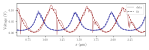
\includegraphics[width=\textwidth]{./chap5/fig/etaTs.pdf}
    \caption{Transmission outcoupling coefficients $\eta_T$ extracted from the fits of the cavity resonances for both cavities I and II as a function of the membrane position. }
    \label{fig:etaTs}
\end{figure}

\subsubsection{Dispersive couplings}
The next essential parameters central to MATE systems are the linear and quadratic dispersive couplings, as developped in chapter II. These are computed from the rescaled scans of the cavity resonances, giving access to the first and second derivative of the peak positions (once rescaled, expressed in FSR units) with respect to the membrane position. These are plotted in Fig \ref{fig:G1G2s}, and we see that, although the second cavity featured a lower finesse, it does display a larger linear dispersive coupling. Due to the different cavity geometry/constraints. These were observed to vary greatly from one cavity to another, independently of the cavity finesse. \\ 


From these various characterization sequences, we extract the key parameters of the two cavities, summarized in Table~\ref{tab:measure_mate_parameters}.
\begin{table}[h!]
    \centering
    \begin{tabular}{lcc}
        & Cavity I & Cavity II \\
        Empty cavity & \quad & \quad  \\
        \hline
        FSR (GHz)                  & 8.817 & 6.246  \\
        Finesse $\mathcal{F}$& 14 000 & 12 780 \\
        Linewidth (kHz)            & 630 & 489\\
        Round-trip loss $T_1 + T_2 + \mathcal{L}$ (ppm) & 449 & 492  \\
        Resonant reflection R(0) & 0.76 & 0.85 \\
        $T_1$ (ppm) & 396 & 455 \\
        $T_2 + \mathcal{L}$ (ppm) & 53 & 37 \\[0.6em]

        MATE cavity & \quad & \quad  \\
        \hline
        Fitted reflectivity $|r_m|$ & 0.54 & 0.33 \\
        Finesse $\mathcal{F}$ &  6 000 - 10 000 &  3 000 - 5 000 \\ 
        Linewidth  (MHz) & 0.88 - 2.20 &  1.25 - 2.10 \\  
        Round-trip loss $T_1 + T_2 + \mathcal{L}_{\text{mem}}$ (ppm) & 630 - 1570 &  1255 - 2095 \\
        Input power        &  10$\mu$W- 50 mW & 10$\mu$W- 50 mW  \\

    \end{tabular}
    \caption{Summary of the measured parameters for the two cavities used in this work.}
    \label{tab:measure_mate_parameters}
\end{table}


\begin{figure}
    \centering  
    \includegraphics[width=\textwidth]{./chap5/fig/G1G2s.pdf}
    \caption{Linear and quadratic dispersive couplings extracted from the rescaled scans of cavity I and II. Units are given in GHz/$\mu$m for $G_1$ and in GHz/$\mu$m$^2$ for $G_2$, as rescaling by the zero point fluctuation in a cavity with a large number of photon obscures the true meaning of the vacuum optomechanical couplings. }
    \label{fig:G1G2s}
\end{figure}

\subsection{Cavity Locking and Mechanical Characterization}
One the cavity was characterized, we proceeded to lock it using the PDH technique detailed in chapter III. The whole lock was done using PyRPL, as to showcase its versatility and ease of use. The analogic signal was manipulated with standard MiniCircuits\textsuperscript{\textregistered} RF components, as to amplify/filter/mix the signals as needed. The overall locking sequence is shown in Fig.~\ref{fig:lock_sequence}, where we can see the various steps needed to lock the cavity. First, performing a fine scan over a cavity resonance as to recover a lorentzian lineshape. From this, we tune the error signal amplitude and demodulation phase as to optimize the PDH error signal (Fig \ref{fig:lock_sequence}(b)). We then engage the lock by first locking on the side of the resonance dip. It was observed that at mW powers, locking on the blue side of the resonance was not feasible. This could be explained by optomechanical heating of the membrane, as changing the side of the lock to the red side made the lock stable. Finally, we engage the PDH lock to lock onto the cavity resonance. The critical point in maintaining the lock was the input power i.e. the cavity circulating power. In terms of power range, locking at 1-50 $\mu$W held the lock, while ramping the input power to 1-50 mW greatly perturbed the optomechanical system such that it was no possible to keep the lock. We suspect that optomechanical heating, bistability and photothermal effects were playing a significant role in the lock stability. \\

Keeping the optical power low, the lock held, and we could proceed to the mechanical characterization of the membrane resonator. Using a spectrum analyzer (Agilent 90A20???), we monitored the spectrum of both the transmitted and reflected intensities. The membrane motion modulating the cavity resonance faster than the lock could respond, the membrane motion modulates the intracavity field intensity, which can in turn be detected in direct detection in both transmission and reflection. The resulting spectra are shown for cavity II in Fig.~\ref{fig:mechproperties}, where we can see the fundamental mechanical resonance at 861kHz, as well as various higher order modes. To reduce the averaging time, we used a Resolution Bandwith (RBW) of 1kHz, which broadens the mechanical peaks, masking the true linewidth from which we could have extracted the effective mechanical quality factor. \\

To extract the intrinsic mechanical quality factor, we then proceeded to do mechanical ringdown measurements. Knowing the mechanical resonance frequencies from the spectra, we excited the membrane motion using the back mirror piezo, while sweeping the cavity. 

\begin{figure}
    \centering  
    \includegraphics[width=\textwidth]{./chap5/fig/lock_sequence.pdf}
    \caption{Lock sequence of the MATE cavity using the PDH technique. (a) Steps of the lock sequence, wgere we launch the side of fringe lock at approcimately -0.3s. The red pitaya then sets its output voltage to 1 and starts PID control as to lock on the 0 of the error signal, which is achieved at time 0s. Being locked at a HWHM from resonance, launching the PDH lock then brings the cavity to resonance at time $\sim$ 0.35s. (b) Zoom on the error signal and reflected intensity during the lock sequence upon prior cavity scan. These traces are used to fine tune the error signal amplitude and demodulation phase as to optimize the PDH error signal. }
    \label{fig:lock_sequence}
\end{figure}


\begin{figure}
    \centering 
    \includegraphics[width=\textwidth]{./chap5/fig/mechproperties.pdf}
    \caption{ }
    \label{fig:mechproperties}
\end{figure}

\begin{figure}
    \centering  
    \includegraphics[width=\textwidth]{./chap5/fig/mech_ringdown.pdf}
    \caption{ }
    \label{fig:mech_ringdown}
\end{figure}


\subsection{Bistability}

\section{Design of an Optomechanical Fibered Cavity}
\subsection{Design considerations}

\vspace{-\baselineskip}

